%==============================================================================
% SIMTiX --- VLSID 2027 submission (6-page IEEE conference format).
% Condensed, floating-point timing-closure-focused variant of simtix.tex.
% Build:  pdflatex simtix_vlsid && pdflatex simtix_vlsid   (twice for xrefs)
% Figures from docs/plot_bench.py into docs/figs/.
%==============================================================================
\documentclass[conference]{IEEEtran}
\IEEEoverridecommandlockouts

\usepackage{cite}
\usepackage{amsmath,amssymb}
\usepackage{graphicx}
\usepackage{booktabs}
\usepackage{xcolor}
\usepackage{tikz}
\usetikzlibrary{positioning,fit,backgrounds,arrows.meta,calc}
\usepackage{url}
\usepackage[hidelinks]{hyperref}

\graphicspath{{../figs/}}

\begin{document}

\title{SIMTiX: A Compact Open-Source SIMT Accelerator for RISC-V\\
with a Pipelined FP32/FP16 Unit and an Interconnect-Bound\\
Timing-Closure Study}

\author{\IEEEauthorblockN{Krishna Gorai}
\IEEEauthorblockA{Indian Institute of Technology Mandi\\
Email: kg05112001@gmail.com}}

\maketitle

\begin{abstract}
We present \textbf{SIMTiX}, a compact, fully-open Single-Instruction
Multiple-Thread (SIMT) accelerator for RISC-V whose entire path---RTL,
simulation, synthesis, place-and-route, and post-route gate-level
sign-off---is reproducible on one workstation. SIMTiX attaches eight lanes
organized into hardware warps to a five-stage RISC-V host through a
memory-mapped offload interface, and implements the full SIMT toolbox:
round-robin warp scheduling with a background memory engine for latency
hiding, cache-line address coalescing, a per-warp reconvergence stack for
control divergence, and an on-chip scratchpad. Placing the vector register
file and scratchpad in distributed RAM (LUTRAM) shrinks the design
$5.7\times$ and closes 100~MHz timing. We extend every lane with a pipelined
floating-point unit in both single and half precision (FP32 and FP16); half
precision reuses the single-precision datapath through NaN-boxed
widen--compute--narrow, which we show is correctly single-rounded and adds no
extra cycles. The unit covers add, multiply, the fused multiply-add, and
iterative divide and square root, verified bit-exact against an IEEE-754
reference over $116{,}089$ vectors. Our central result is a \emph{placed}
timing-closure study of this FP datapath on a Zynq UltraScale+ FPGA. The
FP-enlarged fabric ($2.5\times$ the integer LUTs) is interconnect-bound: a
two-stage FMA closes at only 78~MHz, routing-dominated. We confirm the
diagnosis by de-congestion---a shared serial divide/square-root unit lifts the
placed maximum to 84~MHz with the logic unchanged---and a lane-count
design-space exploration shows the limit is a single lane's intra-lane FMA
cone, not the fabric size. Pipelining that FMA into three stages \emph{meets}
100~MHz and moves the critical path off the floating-point datapath entirely.
The complete RTL, benchmark harness, and FPGA flow are public.
\end{abstract}

\begin{IEEEkeywords}
SIMT, GPGPU, RISC-V, hardware accelerator, floating-point, half precision,
fused multiply-add, timing closure, FPGA, open-source hardware.
\end{IEEEkeywords}

%==============================================================================
\section{Introduction}
%==============================================================================
Graphics processing units execute thousands of scalar threads in lockstep
groups called \emph{warps} under a Single-Instruction Multiple-Thread (SIMT)
model. The mechanisms that make this efficient---warp scheduling for latency
hiding, memory coalescing, control-divergence handling, and on-chip
scratchpads---are well documented for commercial GPUs~\cite{hennessy,aamodt}
but hard to \emph{study in RTL}. Production GPUs are proprietary; open GPGPU
cores such as
Vortex~\cite{vortex} are powerful but large and complex to bring up; and small
academic cores are often simulator-only or stop short of a real implementation
flow.

This paper presents \textbf{SIMTiX}, a deliberately compact open-source SIMT
accelerator for RISC-V whose entire path---RTL through bitstream and post-route
gate-level sign-off---is reproducible on a single workstation with free or
widely available tools. SIMTiX is small enough to read end-to-end yet
implements the complete SIMT mechanism set, and we extend each lane with a
pipelined floating-point unit. Its headline result is a \emph{placed}
timing-closure study showing that, once the lanes carry floating point, the
design becomes \emph{interconnect}-bound rather than logic-bound, and we close
100~MHz by attacking the right lever---the per-lane fused multiply-add
microarchitecture---identified through a measured diagnose--confirm--localize
sequence.

\noindent\textbf{Contributions.}
\begin{itemize}
\item A compact, fully-open SIMT accelerator (eight lanes, four resident warps)
integrated with a five-stage RISC-V host as a self-contained system-on-chip,
exercising the entire RTL-to-bitstream flow
(Sections~\ref{sec:arch}--\ref{sec:impl}).
\item An implementation result showing that moving the vector register file and
scratchpad into distributed RAM reduces LUT usage by $5.7\times$ and closes
100~MHz timing, with a clear analysis of why the register-file read multiplexer,
not the ALUs, dominates a naive SIMT datapath (Section~\ref{sec:impl}).
\item A per-lane floating-point extension covering both FP32 and FP16, in which
half precision is obtained almost for free from the single-precision path via
NaN-boxed widen--compute--narrow (shown to be correctly single-rounded),
verified bit-exact over $116{,}089$ vectors (Section~\ref{sec:fp}).
\item A placed FPGA timing-closure study that diagnoses the FP-enabled design as
interconnect-bound, confirms it by de-congestion, localizes the limit to a single
lane's FMA cone via a lane-count design-space exploration, and closes 100~MHz with
a three-stage FMA that moves the critical path off the FP datapath
(Section~\ref{sec:fppa}).
\end{itemize}

%==============================================================================
\section{SIMTiX Architecture and Platform}\label{sec:arch}
%==============================================================================
A SIMT machine groups scalar \emph{threads} into \emph{warps} that share one
instruction stream and execute on a vector of \emph{lanes}. SIMTiX uses a warp
size equal to its lane count ($\mathrm{WARP\_SIZE}=\mathrm{NUM\_LANES}=8$), with
$\mathrm{NUM\_WARPS}=4$ warps resident and time-sharing a single
fetch/decode/execute datapath; when one warp stalls on memory, the scheduler
issues another, hiding latency. Unlike a packed-SIMD vector unit such as the
RISC-V ``V'' extension~\cite{riscvvector}, where one instruction operates on a
register-resident vector, SIMTiX keeps a scalar thread per lane with an
independent program counter abstraction managed by the reconvergence stack, so
data-dependent control flow is handled in hardware rather than by masking in
software.

SIMTiX is an offload accelerator. The host programs a command block over a
memory-mapped (MMIO) interface---kernel PC, base pointers, thread count
\texttt{N}---writes a \texttt{GO} bit and polls \texttt{DONE}; on \texttt{GO} the
accelerator launches $\lceil N/8\rceil$ warps, seeding each thread's id and
arguments through registers at spawn. Four mechanisms make up the platform.
\emph{Warp pool and scheduler}: four resident slots, each with its own PC, active
mask, register-file partition, and reconvergence stack, share one datapath and
one data port; a round-robin scheduler issues one runnable warp per cycle and a
\emph{background memory engine} services a memory access while other warps' compute
instructions keep the datapath busy. \emph{Coalescing}: the data port is one cache
line wide ($\mathrm{LINE\_WORDS}=8$, 256~bits); the memory engine groups active
lanes' addresses by line and spends one transaction per distinct line, so a
contiguous warp access collapses to a single transaction and a scattered one costs
up to eight. \emph{Reconvergence stack}: each warp owns a SIMT stack whose
top-of-stack frame defines the live PC and active mask; a branch on which active
lanes disagree pushes a frame so the two lane groups run in turn and reconverge at
a join PC, supporting compiler-free single-sided \texttt{if} and divergent loops.
\emph{Scratchpad}: a per-warp 64-word aperture serviced from on-chip RAM lets data
reused across a warp's lanes be staged once, cutting global traffic. The active
mask additionally drives a per-lane clock-enable, so masked-off lanes are not
clocked; the unused-lane fraction is dynamic energy a divergence-aware design
saves (up to 22.5\% on a divergence-heavy kernel)~\cite{gpuwattch}. Every
mechanism is instrumented with hardware counters so it can be measured directly
in RTL, rather than estimated in a software model~\cite{gpgpusim}.

%==============================================================================
\section{Implementation}\label{sec:impl}
%==============================================================================
SIMTiX is written in synthesizable SystemVerilog and integrated with a reused
five-stage RV32I host into a self-contained chip (\texttt{chip\_top},
Fig.~\ref{fig:arch}): host core,
driver ROM, accelerator, and an eight-bank on-chip shared memory. In the
integrated chip the host loads operands into shared memory, launches the
accelerator, and reads results back---the whole
CPU$\rightarrow$memory$\rightarrow$accelerator$\rightarrow$memory$\rightarrow$CPU
loop runs in hardware.

\begin{figure}[t]
\centering
\resizebox{\columnwidth}{!}{%
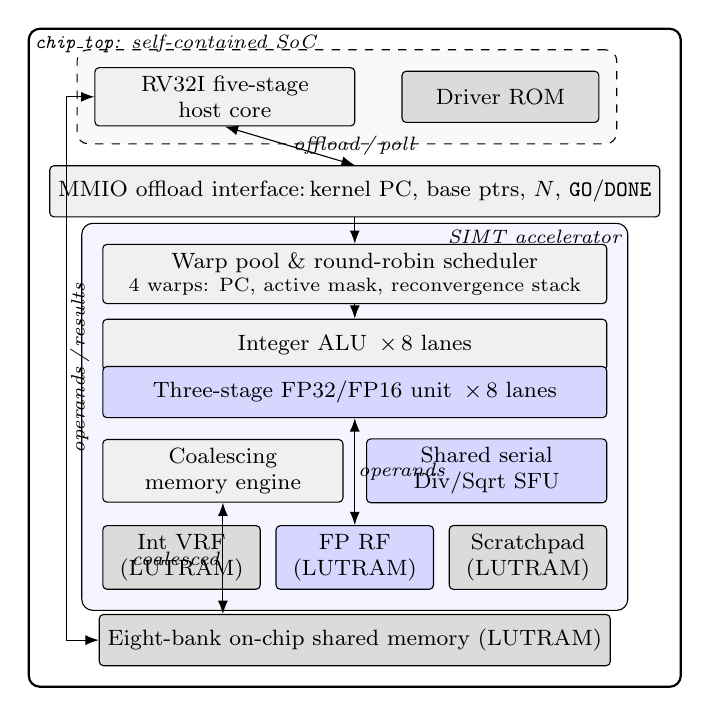
\begin{tikzpicture}[
  font=\footnotesize,
  box/.style={draw,rounded corners=1.5pt,align=center,fill=gray!12,
              inner sep=3pt,minimum height=6.5mm},
  fp/.style ={draw,rounded corners=1.5pt,align=center,fill=blue!16,
              inner sep=3pt,minimum height=6.5mm},
  mem/.style={draw,rounded corners=1.5pt,align=center,fill=gray!28,
              inner sep=3pt,minimum height=6.5mm},
  lab/.style={font=\scriptsize\itshape,inner sep=1pt},
  >=Latex
]
% ---- Host subsystem ----
\node[box,minimum width=3.3cm] (cpu) at (-1.65,7.2) {RV32I five-stage\\host core};
\node[mem,minimum width=2.5cm] (rom) at (1.85,7.2) {Driver ROM};
% ---- MMIO ----
\node[box,minimum width=6.4cm] (mmio) at (0,6.0)
  {MMIO offload interface:\,kernel PC, base ptrs, $N$, \texttt{GO}/\texttt{DONE}};
% ---- Accelerator internals ----
\node[box,minimum width=6.4cm] (sched) at (0,4.95)
  {Warp pool \& round-robin scheduler\\[-1pt]
   {\scriptsize 4 warps: PC, active mask, reconvergence stack}};
\node[box,minimum width=6.4cm] (alu) at (0,4.05) {Integer ALU\, $\times\,8$ lanes};
\node[fp,minimum width=6.4cm]  (fpu) at (0,3.45)
  {Three-stage FP32/FP16 unit\, $\times\,8$ lanes};
\node[box,minimum width=3.05cm] (memeng) at (-1.675,2.45) {Coalescing\\memory engine};
\node[fp,minimum width=3.05cm]  (sfu)    at ( 1.675,2.45) {Shared serial\\Div/Sqrt SFU};
\node[mem,minimum width=2.0cm] (vrf)  at (-2.2,1.35) {Int VRF\\(LUTRAM)};
\node[fp,minimum width=2.0cm]  (frf)  at ( 0.0,1.35) {FP RF\\(LUTRAM)};
\node[mem,minimum width=2.0cm] (spad) at ( 2.2,1.35) {Scratchpad\\(LUTRAM)};
% ---- Shared memory ----
\node[mem,minimum width=6.4cm] (smem) at (0,0.3)
  {Eight-bank on-chip shared memory (LUTRAM)};
% ---- Containers ----
\begin{scope}[on background layer]
  \node[fit=(cpu)(rom),draw,dashed,rounded corners,inner sep=2.2mm,
        fill=gray!5] (hostg) {};
  \node[fit=(sched)(alu)(fpu)(memeng)(sfu)(vrf)(frf)(spad),draw,rounded corners,
        inner sep=2.6mm,fill=blue!4] (accg) {};
  \node[fit=(hostg)(mmio)(accg)(smem),draw,thick,rounded corners,
        inner sep=2.6mm] (chip) {};
\end{scope}
\node[lab,anchor=north east] at ($(accg.north east)+(-0.5mm,-0.5mm)$) {SIMT accelerator};
\node[lab,anchor=north west] at ($(chip.north west)+(0.5mm,-0.5mm)$)
  {\texttt{chip\_top}: self-contained SoC};
% ---- Edges ----
\draw[<->] (cpu.south) -- (mmio.north) node[lab,midway,right] {offload\,/\,poll};
\draw[->]  (mmio.south) -- (sched.north);
\draw[->]  (sched.south) -- (alu.north);
\draw[<->] (fpu.south) -- (frf.north) node[lab,midway,right] {operands};
\draw[<->] (memeng.south) -- (memeng.south|-smem.north)
           node[lab,midway,left] {coalesced};
\draw[<->] (cpu.west) -- ++(-3.5mm,0) |- (smem.west)
           node[lab,pos=0.25,rotate=90,anchor=north] {operands\,/\,results};
\end{tikzpicture}}
\caption{SIMTiX system architecture. The five-stage RISC-V host drives the SIMT
accelerator over a memory-mapped offload interface and exchanges operands and
results through the eight-bank on-chip shared memory; the whole loop is one
self-contained \texttt{chip\_top}. Floating-point blocks (per-lane pipelined
FP32/FP16 unit, FP register file, and the shared serial divide/square-root SFU)
are tinted blue. Register files and the scratchpad live in distributed RAM
(LUTRAM).}
\label{fig:arch}
\end{figure}

\textbf{From flip-flops to LUTRAM.} The first synthesis of the accelerator on a
Zynq UltraScale+ (\texttt{xczu7ev}) consumed 170{,}868 LUTs---74\% of the
device---at only 10\% of its flip-flops. The cause is structural: a flip-flop
vector register file (VRF) of $4\times8\times32$ 32-bit words is 32{,}768
registers read as \texttt{vrf[warp][lane][reg]} with \emph{both} warp and register
variable, i.e.\ a 128-to-1 multiplexer per lane per read port. That multiplexer
fabric, not the ALUs, dominates area and sets the critical path. Re-expressing the
VRF as one distributed-RAM bank per lane (and likewise the scratchpad) removes
essentially all those registers: LUTs fall $5.7\times$ to 30{,}088 (13\%),
flip-flops to 4{,}590 (1.0\%), and the design closes 100~MHz timing with positive
slack at 0.81~W. The complete chip, taken through opt/place/phys-opt/route to a
bitstream, meets all timing at 100~MHz and uses 34{,}850 LUTs (15.1\%), 6{,}130
flip-flops, 24 DSP, and zero BRAM at 1.09~W; the accelerator is $\sim$87\% of the
logic.

\textbf{Verification ladder.} Correctness is established at four levels:
cycle-accurate RTL simulation with self-checking testbenches
(Verilator~\cite{verilator});
behavioral simulation in the vendor GUI; full place-and-route with post-route
timing sign-off; and post-implementation \emph{gate-level} functional simulation
of the routed netlist (UNISIM primitives), which reproduces the integrated chip's
golden checksum of 964 bit-for-bit. The benchmark suite below adds a fifth,
breadth-oriented level.

%==============================================================================
\section{Platform Evaluation}\label{sec:results}
%==============================================================================
We characterize the integer platform with six kernels chosen to stress distinct
mechanisms: \texttt{vadd} ($C_i=A_i+B_i$, streaming), \texttt{saxpy}
($3A_i+B_i$, coalescing), \texttt{fir} ($A_i+2A_{i+1}+A_{i+2}$, stencil),
\texttt{relu} (light divergence), \texttt{collatz} (heavy data-dependent
divergence), and \texttt{reduce} (scratchpad reduction). Each is assembled from
RISC-V source with a stock toolchain, run at $N\in\{8,64,256,1024\}$ threads, and
checked bit-exact against a golden model. For an apples-to-apples speedup, each
kernel is also written as a scalar loop and run on the \emph{same} five-stage host
in RTL.

Table~\ref{tab:speedup} gives the headline platform result. Throughput ramps with
occupancy (latency hiding) and saturates near 6.7 work-items/cycle---below the
eight-lane ideal because of the single shared data port. Streaming kernels reach
$7$--$10\times$ over the scalar host; \texttt{fir} is lower ($7.0\times$) due to
its stencil's partial coalescing; \texttt{collatz} achieves $2.8\times$ as heavy
divergence erodes---but does not eliminate---the SIMT advantage; and
\texttt{reduce} falls below break-even ($0.72\times$), reported honestly---a
single-lane collapse on a single-ported scratchpad is slower than the scalar core
and wants a dedicated cross-lane reduction primitive. SIMTiX is parameterized in
its lane and warp counts; a sweep over $\mathrm{NUM\_LANES}\in\{4,8,16,32\}$ and
$\mathrm{NUM\_WARPS}\in\{2,4,8\}$ (all twelve elaborate and verify bit-exact) shows
throughput scaling near-linearly with lanes ($\sim\!1.97\times$ per doubling) while
the resident-warp count makes little difference under the single-cycle behavioral
memory model---occupancy beyond two warps pays off only under realistic multi-cycle
memory.

\begin{table}[t]
\caption{Measured cycles and speedup over the five-stage RV32I host running
identical work (largest size; \texttt{collatz} at $N{=}256$). Lane utilization
from the accelerator counters.}
\label{tab:speedup}
\centering
\footnotesize
\begin{tabular}{lrrrrr}
\toprule
Kernel & $N$ & Accel & CPU & Speedup & Lane-util\\
\midrule
\texttt{vadd}    & 1024 & 1{,}413 & 13{,}322 & $9.43\times$ & 100\%\\
\texttt{saxpy}   & 1024 & 1{,}669 & 16{,}394 & $9.82\times$ & 100\%\\
\texttt{fir}     & 1024 & 2{,}053 & 14{,}345 & $6.99\times$ & 100\%\\
\texttt{relu}    & 1024 & 1{,}284 & 12{,}809 & $9.98\times$ & 93.7\%\\
\texttt{collatz} &  256 & 9{,}637 & 26{,}601 & $2.76\times$ & 68.3\%\\
\texttt{reduce}  & 1024 & 6{,}023 &  4{,}363 & $0.72\times$ & 39.8\%\\
\bottomrule
\end{tabular}
\end{table}

%==============================================================================
\section{Floating-Point Extension}\label{sec:fp}
%==============================================================================
The base engine is integer-only. We extend it with floating point in both single
(FP32) and half (FP16) precision, keeping the same SIMT structure: the extension
is a per-lane execute unit and a second per-lane register file, not a new
pipeline. Each lane gains a compact fixed-latency FP unit beside its integer ALU,
and a second per-lane register file holds the 32 floating-point registers in
distributed RAM, addressed by \{warp, register\} exactly like the integer VRF, with
an independent write port so an FP result and an integer load can retire together.
The unit implements add, subtract, multiply, the fused multiply-add (all four sign
variants), sign-injection, min/max, the ordered compares,
integer$\leftrightarrow$float and FP32$\leftrightarrow$FP16 conversion, the
bit-moves, and classify, in both precisions; rounding is round-to-nearest-even
per IEEE~754~\cite{ieee754} and subnormals are flushed to zero, a
throughput-oriented choice that keeps each lane
small.

\textbf{Half precision via widen--compute--narrow.} A 16-bit half lives in a
32-bit register NaN-boxed (upper 16 bits all ones); a mis-boxed value reads as a
canonical NaN per the RISC-V convention~\cite{riscv}. For an FP16 operation the unit widens the
operand exactly to FP32, runs the single-precision datapath, and rounds back to
FP16. This is correct, not approximate: because the FP32 intermediate carries a
24-bit significand and $24 \ge 2\cdot 11 + 2$, rounding first to FP32 and then to
FP16 equals rounding directly to FP16~\cite{figueroa}, so FP16 add/sub/mul, the
fused multiply-add, and conversions are correctly single-rounded. Half precision
thus reuses the verified single-precision logic almost entirely, adding only the
widen, narrow, and box steps---and, as Fig.~\ref{fig:fpthr} shows, no extra cycles.

\textbf{Fused multiply-add.} The FMA computes $\pm(a\cdot b)\pm c$ with a
\emph{single} rounding~\cite{muller}, so it cannot be built by chaining the
multiplier and adder.
The unit forms the exact 48-bit product, anchors it in a wide fixed-point
accumulator, aligns the addend while capturing a sticky bit, and normalizes and
rounds once; when the addend out-ranges the product beyond the rounding window the
product is provably below half a ulp, giving the addend exactly and bounding the
alignment shifter. It has fixed latency and commits through the ordinary writeback
path; Section~\ref{sec:fppa} describes how this combinational chain is pipelined
for timing closure.

\textbf{Multi-cycle divide and square root.} Division and square root are produced
one quotient/root bit per cycle by a digit-recurrence~\cite{ercegovac}---the
engine's only multi-cycle operations. Because such a core is comparatively large, the engine has
a \emph{single shared} one: when a warp issues a divide or square root the engine
captures all its lanes' operands and parks the warp on a stall scoreboard, then
sequences the active lanes through the shared core one at a time---the same
park-and-resume mechanism the memory engine uses, so the scheduler keeps issuing
other warps onto the idle datapath meanwhile. At most one warp's divide/square root
is in flight, trading latency ($k$ active lanes take $\sim\!k$ times as long, hidden
across warps) for the area saving quantified in Section~\ref{sec:fppa}.

\textbf{Verification.} Each unit is verified standalone against a DPI-C IEEE-754
reference: FP32 against the host's correctly-rounded \texttt{float} operations
(including \texttt{fmaf} and \texttt{sqrtf}), and FP16 against a \texttt{double}-based
reference cross-checked with \texttt{\_Float16}. Over random vectors spanning the
product-dominant, balanced (cancellation), and addend-dominant regimes plus directed
infinity/NaN/zero/flush/overflow, divide-by-zero, square-root-of-negative,
mis-boxed-operand, and conversion corners, the pipelined unit passes $96{,}066$
checks and the iterative divide/square-root unit a further $20{,}023$, all bit-exact
(Table~\ref{tab:fpverif}). End-to-end FP kernels then run the full warp pool:
streaming add and multiply-add in each precision, a fused $C_i=A_iB_i+C_i$, and
$C_i=\sqrt{A_i/B_i}$ (two dependent multi-cycle ops per thread), all bit-exact to
1024 threads.

\begin{table}[t]
\caption{Floating-point operation coverage. Every operation is implemented and
checked in both FP32 and FP16; all checks are bit-exact against an IEEE-754
reference.}
\label{tab:fpverif}
\centering
\footnotesize
\begin{tabular}{ll}
\toprule
Category & Operations (each in FP32 \emph{and} FP16)\\
\midrule
Arithmetic     & \texttt{fadd}, \texttt{fsub}, \texttt{fmul}\\
Fused          & \texttt{fmadd}, \texttt{fmsub}, \texttt{fnmsub}, \texttt{fnmadd}\\
Divide / root  & \texttt{fdiv}, \texttt{fsqrt} (iterative, multi-cycle)\\
Sign / select  & \texttt{fsgnj\{,n,x\}}, \texttt{fmin}, \texttt{fmax}\\
Compare        & \texttt{feq}, \texttt{flt}, \texttt{fle}\\
Convert        & float$\leftrightarrow$int (signed/unsigned), FP32$\leftrightarrow$FP16\\
Move / classify& \texttt{fmv.x.\_}, \texttt{fmv.\_.x}, \texttt{fclass}\\
\midrule
\multicolumn{2}{l}{Bit-exact checks vs IEEE reference:
\textbf{116{,}089} (0 mismatches)}\\
\bottomrule
\end{tabular}
\end{table}

\textbf{FP throughput and application kernels.} The FP unit is pipelined
(Section~\ref{sec:fppa}); an FP instruction commits a fixed number of cycles after
issue and the issuing warp parks a single slot until it does, latency that SIMT
interleaving hides on streaming work. Figure~\ref{fig:fpthr} plots throughput
versus problem size for streaming add and multiply-add in both precisions: the same
latency-hiding ramp as the integer suite, saturating near 7 work-items/cycle at
100\% lane utilization, with the FP16 curves lying exactly on the FP32 ones---half
precision shares the pipelined datapath and costs no extra time.
Table~\ref{tab:fpkernels} runs four toolchain-assembled FP kernels through the
engine. Two effects stand out: the iterative divide/square-root unit is visible
(\texttt{fnorm}$=A/\sqrt{B}$ takes $\sim\!6\times$ the cycles of streaming
\texttt{fsaxpy}, the honest price of correctly-rounded SFU operations), and
divergence interacts with the now-larger lane datapath (\texttt{fdot}'s reduction
leaves one of eight lanes active during the collapse, $45\%$ utilization, so the
absolute energy a mask-gated design saves grows with the FP-enlarged lane).

\begin{figure}[t]
\centering
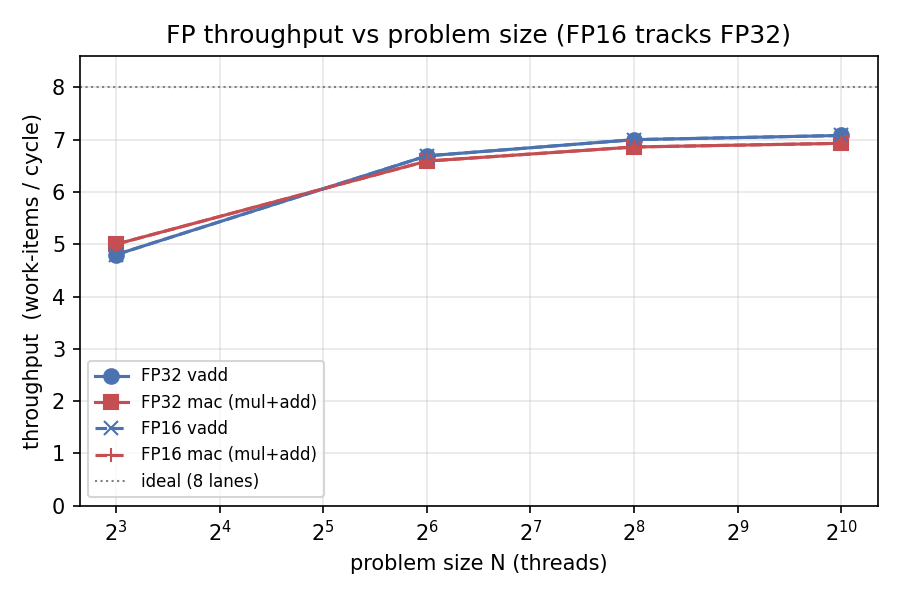
\includegraphics[width=\columnwidth]{fp_throughput.png}
\caption{Floating-point throughput versus problem size for streaming add and
multiply-add kernels. The ramp is the same latency-hiding behavior as the integer
suite; the FP16 curves coincide with the FP32 ones because both use the same
pipelined datapath.}
\label{fig:fpthr}
\end{figure}

\begin{table}[t]
\caption{FP application kernels (FP32 unless noted), verified bit-exact. Cycles,
global line transactions, and lane utilization at $N{=}256$.}
\label{tab:fpkernels}
\centering
\footnotesize
\begin{tabular}{llrrr}
\toprule
Kernel & Computation & Cycles & Gmem & Lane-util\\
\midrule
\texttt{fsaxpy}   & $\alpha A_i + B_i$ (fmadd) & 419  & 96 & 100\%\\
\texttt{fsaxpy16} & $\alpha A_i + B_i$ (FP16)  & 451  & 96 & 100\%\\
\texttt{fnorm}    & $A_i/\sqrt{B_i}$ (div+sqrt)& 2{,}396 & 96 & 100\%\\
\texttt{fdot}     & $\sum_l A_{8w+l}B_{8w+l}$  & 1{,}991 & 96 & 45\%\\
\bottomrule
\end{tabular}
\end{table}

%==============================================================================
\section{Placed Timing Closure of the FP Datapath}\label{sec:fppa}
%==============================================================================
Floating point raises the accelerator from 30{,}088 to 74{,}342 LUTs
($2.5\times$), flip-flops from 4{,}590 to 7{,}894, and DSP blocks from 24 to 40
(the FP multipliers), at 1.34~W. The increase is dominated by the common-case
arithmetic unit---eight per-lane copies of the add/multiply/FMA/convert datapath,
the fused multiply-add the largest single block---not the iterative
divide/square-root cores, which synthesize to only $689$ LUTs each
($\sim$7\% of the design). The FMA is also the longest combinational chain: as a
single-cycle block its raw path is 16.2~ns (61~MHz), making it the frequency
bottleneck. Table~\ref{tab:fpclose} summarizes the placed utilization and frequency
of each step in the closure; we walk through them.

\textbf{Two-stage FMA (78~MHz, interconnect-bound).} We first pipeline the FP unit
into two stages, split at the FMA accumulator (\texttt{mag}) boundary; the warp
pool absorbs the extra cycle with a single-slot scoreboard (\texttt{W\_FPC}), the
same park-and-resume mechanism used for memory and the SFU, so no new structural
hazard arises and SIMT interleaving hides the latency. Timing-driven synthesis with
retiming cuts the FP \emph{logic} depth to 5.3~ns, yet place-and-route closes at
12.8~ns (\textbf{78~MHz}). The placed critical path is still the first FMA stage but
now \emph{routing}-dominated---7.4 of 12.8~ns (58\%) is wire delay---because in the
FP-enlarged fabric ($2.5\times$ the integer LUTs across eight wide FP lanes)
interconnect, not logic depth, has become the binding constraint.

\textbf{Confirming the diagnosis (84~MHz).} If congestion is the limit,
de-congesting the fabric should raise frequency with the logic unchanged. We fold
the eight per-lane divide/square-root cores into a single shared serial unit, fed
lane-by-lane. This removes $\sim$3.7k LUTs and $\sim$1.2k flip-flops and drops power
from 1.53 to 1.22~W; crucially it leaves the FMA critical path structurally
unchanged yet cuts that path's \emph{routing} delay from 7.4 to 6.5~ns, raising the
placed maximum to \textbf{84~MHz} and reducing near-critical endpoints from 8.7k to
3.2k. Same logic, less congestion, higher frequency---a direct confirmation that
interconnect, not logic depth, bounds this design.

\textbf{Localizing the limit: frequency does not scale with fabric size.} A natural
question is whether \emph{trimming} the FP fabric relieves congestion further. It
does not. Placing the design at four lanes (Table~\ref{tab:fpclose}, last row)
halves its area---37k versus 69k LUTs, 20 versus 40 DSPs---but reaches only
79.7~MHz, marginally \emph{below} the eight-lane 84.1~MHz, and the router still
reports CLB congestion. The critical path is a \emph{single} lane's FMA cone, whose
logic depth and locally-dense 128-bit datapath are independent of the lane count;
halving the lanes replicates that cone fewer times but packs the smaller design
into a denser region that gives the lone FMA no relief. The eight-lane configuration
thus Pareto-dominates the four-lane one (equal frequency, twice the throughput) and
identifies the true frequency lever as the FMA \emph{microarchitecture}, not the
fabric size.

\textbf{Closing 100~MHz: a three-stage FMA.} Acting on that finding, we split the
FMA across \emph{three} stages---product, 128-bit align-and-add, and
normalize-and-round---so no single stage carries the whole cone. The warp pool
absorbs the extra cycle with the same single-slot scoreboard, now a two-cycle
writeback latency that SIMT interleaving continues to hide on streaming work; the
added registers raise flip-flops to 15.0k while leaving LUTs (70.0k), DSPs, power
(1.22~W), and the bit-exact results unchanged. Place-and-route now \emph{meets}
timing at 100~MHz (worst setup slack $+0.071$~ns;
Table~\ref{tab:fpclose} traces $78\rightarrow84\rightarrow100.7$~MHz across the
three steps), and decisively the critical path moves \emph{off} the FMA onto the
vector-register-file LUTRAM read mux---the same structure that bounds the
\emph{integer} design (Section~\ref{sec:impl}). The floating-point datapath is no
longer the frequency limiter, confirming that FMA logic depth---the lever the
design-space exploration identified---was the true constraint all along.

\begin{table*}[t]
\caption{Placed post-route PPA of the FP-enabled accelerator across the
timing-closure steps and the lane design-space point (\texttt{xczu7ev},
out-of-context place-and-route, 100~MHz constraint). Steps~1--3 hold the lane count
at eight and progressively pipeline the datapath; the final row (DSE) trims to four
lanes. Pipelining the FMA from two to three stages (step~3) is what meets 100~MHz
and moves the critical path off the FP datapath; the shared SFU (step~2) and lane
trimming (DSE) help area and power but not the frequency floor. LUTRAM is the
distributed-RAM subset of the LUT count; the design uses zero block RAM throughout.
Utilization percentages are of the \texttt{xczu7ev} (230{,}400 LUTs, 460{,}800 FFs,
1{,}728 DSPs).}
\label{tab:fpclose}
\centering
\footnotesize
\begin{tabular}{llrrrrrrrrl}
\toprule
\# & FP datapath & Lanes & LUT & LUTRAM & FF & DSP & BRAM & Power & Fmax & Crit.\ path\\
   &             &       & (31\%) &       & (3\%) & (2\%) & & (W) & (MHz) & \\
\midrule
1 & Two-stage FMA          & 8 & 72{,}573 & 3{,}348 & 12{,}347 & 40 & 0 & 1.53 & 78.0  & FMA cone\\
2 & {}+ shared serial SFU  & 8 & 68{,}914 & 3{,}348 & 11{,}153 & 40 & 0 & 1.22 & 84.1  & FMA cone\\
3 & Three-stage FMA        & 8 & 69{,}987 & 3{,}348 & 14{,}954 & 40 & 0 & 1.22 & \textbf{100.7} & VRF LUTRAM\\
\midrule
  & \emph{DSE:} four lanes & 4 & 36{,}785 & 1{,}748 &  6{,}953 & 20 & 0 & 0.98 & 79.7  & FMA cone\\
\bottomrule
\end{tabular}
\end{table*}

%==============================================================================
\section{Related Work}\label{sec:related}
%==============================================================================
Open RISC-V GPGPU cores include Vortex~\cite{vortex}, a full OpenCL-capable
multi-core design, and Ventus~\cite{ventus}, a PTX/Vortex-style GPGPU; both target
performance and scale and are correspondingly large. Simty~\cite{simty}
demonstrates generalized SIMT execution of the RISC-V ISA, and Nyuzi~\cite{nyuzi}
is a synthesizable vector GPGPU for graphics research. Open floating-point units
such as FPnew~\cite{fpnew} offer multiformat arithmetic as standalone IP; SIMTiX
instead integrates a per-lane FP datapath into the SIMT pipeline and studies its
\emph{placed} timing. Relative to these, SIMTiX is deliberately small and readable,
and its contribution is not raw performance but a complete, reproducible
RTL-to-bitstream flow paired with a placed timing-closure study of a SIMT
floating-point datapath---a result, the interconnect-bound nature of an FP-enlarged
SIMT fabric and the FMA-microarchitecture lever that closes it, that the larger
cores do not report. Control-divergence handling via reconvergence stacks is long
studied~\cite{fung,tesla}; we use the standard stack mechanism and reuse its mask
for lane clock-gating.

%==============================================================================
\section{Conclusion}
%==============================================================================
SIMTiX shows that the full SIMT mechanism set fits in a compact, fully-open RISC-V
accelerator that runs end-to-end through a real implementation flow, with a
distributed-RAM register file the key to making it small and fast on FPGA. A
per-lane floating-point unit adds FP32 and FP16 arithmetic---including the fused
multiply-add and iterative divide/square root---with half precision obtained almost
for free from the single-precision path and verified bit-exact over $116{,}089$
vectors. The central result is a placed timing-closure study: the FP-enlarged
fabric is interconnect-bound, a fact we diagnose, confirm by de-congestion, and
localize to a single lane's FMA cone, then close 100~MHz with a three-stage FMA that
moves the critical path off the floating-point datapath onto the same
register-file read mux that bounds the integer design. The remaining headroom is in
that shared mux; an open-source ASIC path through the SkyWater~130\,nm
PDK~\cite{sky130} with OpenLane~\cite{openlane} would turn these FPGA numbers into
silicon-relevant area, frequency, and power. The design and its evaluation
infrastructure are public, so the results are reproducible and the platform is
reusable for teaching and research.

%==============================================================================
\begin{thebibliography}{99}
\bibitem{vortex} B.~Tine, K.~P.~Yalamarthy, F.~Elsabbagh, and H.~Kim,
``Vortex: Extending the RISC-V ISA for GPGPU and 3D-Graphics,'' in
\emph{Proc. IEEE/ACM MICRO}, 2021.
\bibitem{ventus} F.~Zhang \emph{et al.}, ``Ventus: a RISC-V based GPGPU,''
open-source project, 2022.
\bibitem{simty} S.~Collange, ``Simty: Generalized SIMT execution on RISC-V,''
in \emph{Workshop on Computer Architecture Research with RISC-V (CARRV)}, 2017.
\bibitem{nyuzi} J.~Bush, P.~Dexter, T.~N.~Miller, and A.~Carpenter,
``Nyami: a synthesizable GPU architectural model for general-purpose and
graphics-specific workloads,'' in \emph{Proc. IEEE ISPASS}, 2015.
\bibitem{fung} W.~W.~L.~Fung, I.~Sham, G.~Yuan, and T.~M.~Aamodt,
``Dynamic Warp Formation and Scheduling for Efficient GPU Control Flow,'' in
\emph{Proc. IEEE/ACM MICRO}, 2007.
\bibitem{tesla} E.~Lindholm, J.~Nickolls, S.~Oberman, and J.~Montrym,
``NVIDIA Tesla: A Unified Graphics and Computing Architecture,''
\emph{IEEE Micro}, vol.~28, no.~2, 2008.
\bibitem{aamodt} T.~M.~Aamodt, W.~W.~L.~Fung, and T.~G.~Rogers,
\emph{General-Purpose Graphics Processor Architectures}. Morgan \& Claypool,
2018.
\bibitem{hennessy} J.~L.~Hennessy and D.~A.~Patterson, \emph{Computer
Architecture: A Quantitative Approach}, 6th ed. Morgan Kaufmann, 2017.
\bibitem{gpgpusim} A.~Bakhoda, G.~L.~Yuan, W.~W.~L.~Fung, H.~Wong, and
T.~M.~Aamodt, ``Analyzing CUDA Workloads Using a Detailed GPU Simulator,'' in
\emph{Proc. IEEE ISPASS}, 2009.
\bibitem{gpuwattch} J.~Leng \emph{et al.}, ``GPUWattch: Enabling Energy
Optimizations in GPGPUs,'' in \emph{Proc. ACM/IEEE ISCA}, 2013.
\bibitem{fpnew} S.~Mach, F.~Schuiki, F.~Zaruba, and L.~Benini, ``FPnew: An
Open-Source Multiformat Floating-Point Unit Architecture for Energy-Proportional
Transprecision Computing,'' \emph{IEEE Trans. VLSI Syst.}, vol.~29, no.~4,
pp.~774--787, 2021.
\bibitem{riscv} A.~Waterman and K.~Asanovi\'c, ``The RISC-V Instruction Set
Manual, Volume I: Unprivileged ISA,'' RISC-V International, 2019.
\bibitem{riscvvector} RISC-V International, ``RISC-V ``V'' Vector Extension,
Version 1.0,'' specification, 2021.
\bibitem{ieee754} IEEE, ``IEEE Standard for Floating-Point Arithmetic,''
\emph{IEEE Std 754-2019}, 2019.
\bibitem{muller} J.-M.~Muller \emph{et al.}, \emph{Handbook of Floating-Point
Arithmetic}, 2nd ed. Birkh\"auser, 2018.
\bibitem{ercegovac} M.~D.~Ercegovac and T.~Lang, \emph{Digital Arithmetic}.
Morgan Kaufmann, 2004.
\bibitem{figueroa} S.~A.~Figueroa, ``When is double rounding innocuous?,''
\emph{ACM SIGNUM Newsletter}, vol.~30, no.~3, pp.~21--26, 1995.
\bibitem{verilator} W.~Snyder, ``Verilator: Open-Source SystemVerilog
Simulation and Verification,'' Veripool, \url{https://www.veripool.org/verilator}.
\bibitem{sky130} SkyWater Technology and Google, ``SkyWater Open Source PDK
(sky130),'' \url{https://github.com/google/skywater-pdk}.
\bibitem{openlane} A.~Ghazy and M.~Shalan, ``OpenLane: The Open-Source Digital
ASIC Implementation Flow,'' in \emph{Workshop on Open-Source EDA Technology
(WOSET)}, 2020.
\end{thebibliography}

\end{document}
